\documentclass[a4paper]{report}

% --- PACKAGES DE BASE ---
\usepackage[utf8]{inputenc}
\usepackage[T1]{fontenc}
\usepackage[french]{babel}
\usepackage[left=2.5cm, right=2.5cm, top=2.5cm, bottom=2.5cm]{geometry}

% --- GRAPHISMES ET MISE EN PAGE ---
\usepackage{graphicx}
\usepackage{float}
\usepackage{xcolor}
\usepackage{tikz}
\usepackage{background}
\usepackage{pdfpages}
\usepackage{wrapfig}
\usepackage{array}

% --- TITRES ET SOMMAIRE ---
\usepackage{titlesec}
\usepackage{tocloft}

% --- OUTILS SUPPLÉMENTAIRES ---
\usepackage{amsmath}
\usepackage{lipsum}
\usepackage{verbatim}
\usepackage[colorlinks=true, linkcolor=blue, citecolor=green]{hyperref}

% --- BIBLIOGRAPHIE ---
\usepackage[backend=biber, style=numeric]{biblatex} 
\addbibresource{references.bib}

% --- CONFIGURATION LISTINGS (CODE) ---
\usepackage{listings}
\definecolor{codegreen}{rgb}{0,0.6,0}
\definecolor{codegray}{rgb}{0.5,0.5,0.5}
\definecolor{codepurple}{rgb}{0.58,0,0.82}
\definecolor{backcolour}{rgb}{0.95,0.95,0.92}

\lstdefinestyle{pythonstyle}{
    backgroundcolor=\color{backcolour},
    commentstyle=\color{codegreen},
    keywordstyle=\color{blue},
    numberstyle=\tiny\color{codegray},
    stringstyle=\color{codepurple},
    basicstyle=\ttfamily\footnotesize,
    breaklines=true,
    captionpos=b,
    keepspaces=true,
    numbers=left,
    numbersep=5pt,
    showspaces=false,
    showstringspaces=false,
    showtabs=false,
    tabsize=2,
    language=Python,
    literate={é}{{\'e}}1 {è}{{\`e}}1 {à}{{\`a}}1 {ç}{{\c{c}}}1 {œ}{{\oe}}1 {ù}{{\`u}}1 {É}{{\'E}}1 {È}{{\`E}}1 {À}{{\`A}}1 {°}{{$^\circ$}}1
}
\lstset{style=pythonstyle}

% --- CONFIGURATION DES TITRES ---
\titlespacing*{\chapter}{0pt}{-20pt}{30pt}
\titleformat{\chapter}[display]
  {\normalfont\Huge\bfseries} % Taille pour "Chapitre X"
  {\chaptertitlename\ \thechapter}
  {10pt}                      % Espace entre le numéro et le titre (réduit ici)
  {\huge}                     % Taille pour le nom du titre (modifié de \Huge à \huge)

\renewcommand{\contentsname}{Table des matières}

% --- DÉBUT DU DOCUMENT ---
\begin{document}

% 1. Page de garde (via PDF externe)
\backgroundsetup{contents={}}

\includepdf[pages=-, fitpaper=true]{Template.pdf}

% 2. Configuration du fond pour le reste du document
\backgroundsetup{
    scale=1,
    angle=0,
    opacity=1,
    color=black,
    contents={
        \begin{tikzpicture}[remember picture,overlay]
        \node at ([xshift=-0.8in,yshift=0.8in] current page.south east) {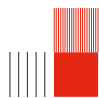
\includegraphics[scale=0.8]{images/pattern.png}};
        \end{tikzpicture}
    }
}

% 3. Remerciements
\clearpage
\thispagestyle{empty}
\vspace*{\fill}
\section*{Remerciements}
\addcontentsline{toc}{chapter}{Remerciements}
Ce projet multidisciplinaire n'aurait pu voir le jour sans l'aide de...
\vspace*{\fill}

% 4. Abstract
\clearpage
\thispagestyle{empty}
\vspace*{\fill}
\section*{Abstract}
\addcontentsline{toc}{chapter}{Abstract} % Corrigé ici
Ce document est le rapport final du projet... 
\vspace*{\fill}

% 5. Sommaire et Contenu
\clearpage
\tableofcontents

\chapter{Introduction}
\section{Contexte}
Le projet porte sur le quadrupôle d'Okayama...

\chapter{Théorie physique}
\section{Principe de moindre action}
En optique des particules chargées, l'équivalent du principe de Fermat est le principe de moindre action.
Celui-ci s'exprime comme 

\begin{equation}
\begin{aligned}
\delta S = \int_{S0}^{S1} \vec{p}\,\frac{\vec{r}}{dS} \, \mathrm{d}s = 0
\end{aligned}
\end{equation}
\\
Ce principe peut être réecrit en utilisant l'indice optique. On a alors 

\begin{equation}
\begin{aligned}
\delta S = \int_{S0}^{S1} \mu\,\mathrm{d}z = 0
\end{aligned}
\end{equation}
\\
Comme le quadrupole que nous utilisons est composé UNIQUEMENT de lentilles électrostatiques, on peut écrire

\begin{equation}
\begin{aligned}
\mu = \sqrt{\phi(1+(x')^2 + (y')^2)}
\end{aligned}
\end{equation}

avec $\mu$ l'indice optique, $\phi$ le potentiel électrostatique et x' et y' les dérivées de x et y par
rapport à z.
\\
\\
Afin de pouvoir retrouver la trajectoire des particules chargées qui passent à travers le système, il faut 
retrouver l'indice optique du système. Cela est faisable en retrouvant le potentiel électrostatique dans tout le volume du
système et la vitesse des particules dans les directions x et y. 

\section{Equations d'Euler-Lagrange}
Les équations d'Euler-Lagrange sont des équations équivalentes au principe de moindre action, sous forme 
différentielle. On peut ainsi noter 

\begin{equation}
\begin{aligned}
\frac{\partial \mu}{\partial x}-\frac{d}{dz}\left(\frac{\partial \mu}{\partial x'}\right)=0\\
\frac{\partial \mu}{\partial y}-\frac{d}{dz}\left(\frac{\partial \mu}{\partial y'}\right)=0
\end{aligned}
\end{equation}


\section{Extraction du potentiel}
Afin de pouvoir retrouver le potentiel électrostatique en tout point du volume du système, on utilise une 
méthode mathématique: la méthode des éléments de frontières. En anglais, cette méthode se nomme Boundary 
Element Method (BEM). 
\\
\\
{\color{red}
--> Il faut détailler mais je sais pas quoi dire }
\\
\\
Une fois le potentiel extrait en tout point de l'espace, il est utile de décomposer celui-ci afin de pouvoir séparer les 
différentes composantes en fonction de leur dépendance aux différents ordres de x et y. On peut montrer que le potentiel s'exprime 
alors comme 

\begin{equation}
\begin{aligned}
\boxed{
\phi ({\color{red}r},{\color{blue}\theta},{\color{green}z})= \sum\limits_{\nu =0}^{\infty}
\sum\limits_{\lambda=0}^{\infty} \frac{(-1)^{\lambda}\times (\nu !)}{4^{\lambda}\times \lambda !\times (\lambda +\nu)!}
\times {\color{red}r}^{\nu +2\lambda} \times \left(\Phi_{\nu {r}}^{[2\lambda]}({\color{green}z})\times cos(\nu{\color{blue}\theta}) \right)}
\end{aligned}
\end{equation}
\\
En injectant l'expression précédente dans les équations d'Euler-Lagrange, on obtient les équations différentielles suivantes, appelées équations de la trajectoire
\begin{equation}
\begin{aligned}
x''(z) + \frac{\phi'_0(z)}{2\phi_0}x'(z) + \left( \frac{\phi_0''(z)}{4\phi_0(z)} -
\frac{\phi_2(z)}{\phi_0(z)}\right) x(z) = 0 \\
y''(z) + \frac{\phi'_0(z)}{2\phi_0}y'(z) + \left(\frac{\phi_0''(z)}{4\phi_0(z)} +
\frac{\phi_2(z)}{\phi_0(z)}\right) y(z) = 0
\end{aligned}
\end{equation}
\\
\\
Comme leur nom l'indique, la  résolution des équations suivantes à l'aide de la méthode mathématique Runge-Kutta 4, on retrouve la trajectoire des 
particules chargées à travers le système. 

\chapter{Application}
Le but de ce projet multidisciplinaire est de modéliser un quadrupole électrostatique. Pour cela, plusieurs étapes clés sont nécessaires: modélisation de la géométrie, extraction du 
potentiel électrostatique, décomposition du potentiel et résolution des équations de la trajectoire. 
\begin{figure}[H]
\centering
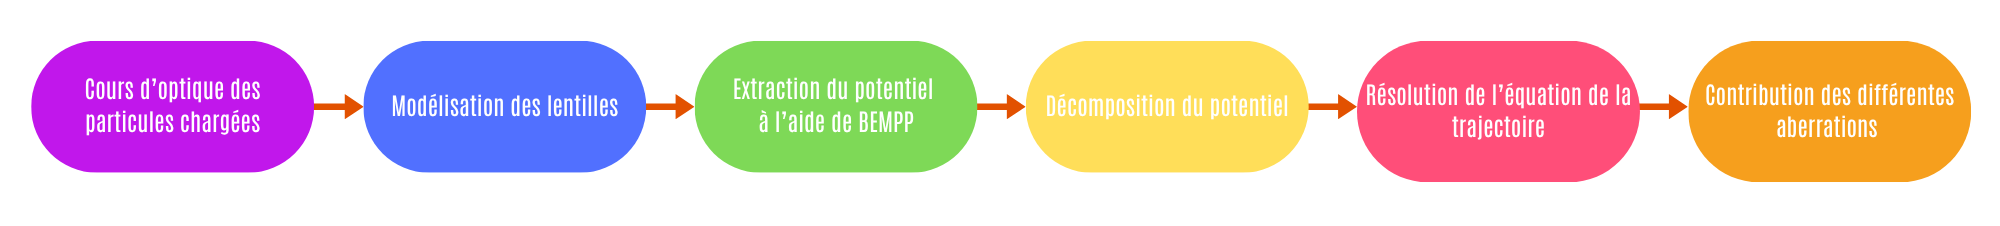
\includegraphics[width=1\linewidth]{images/Logigramme.png} 
\caption{Logigramme présentant les différentes étapes du projet}
\label{fig:Logigramme}
\end{figure}
\section{Modélisation du quadrupole d'Okayama}
Afin de pouvoir utiliser la méthode des éléments de frontière, il faut mailler la géométrie du quadrupole que nous souhaitons modéliser. Ce maillage est fait en utilisant une
extension en bibliothèque Python du générateur de maillage open-source Gmsh.
\\
\\
{\color{red}
--> Penser à créditer}
\\
\\
Au début du projet, nous nous sommes appuyées sur le projet multidisciplinaire de Niels BRUN et Paul BESNARD. Le but de ce projet était de modéliser 
des lentilles de Einzel. Ces lentilles sont trois électrodes circulaires trouées au centre. Les électrodes extérieures sont à la masse tandis que 
l'électrode du centre est polarisée. Ces lentilles servent dans le système de lentilles condenseurs. 
Afin de prendre en main la bibliothèque Gmsh, nous avons modélisé des lentilles de Einzel.

\begin{figure}[H]
\centering
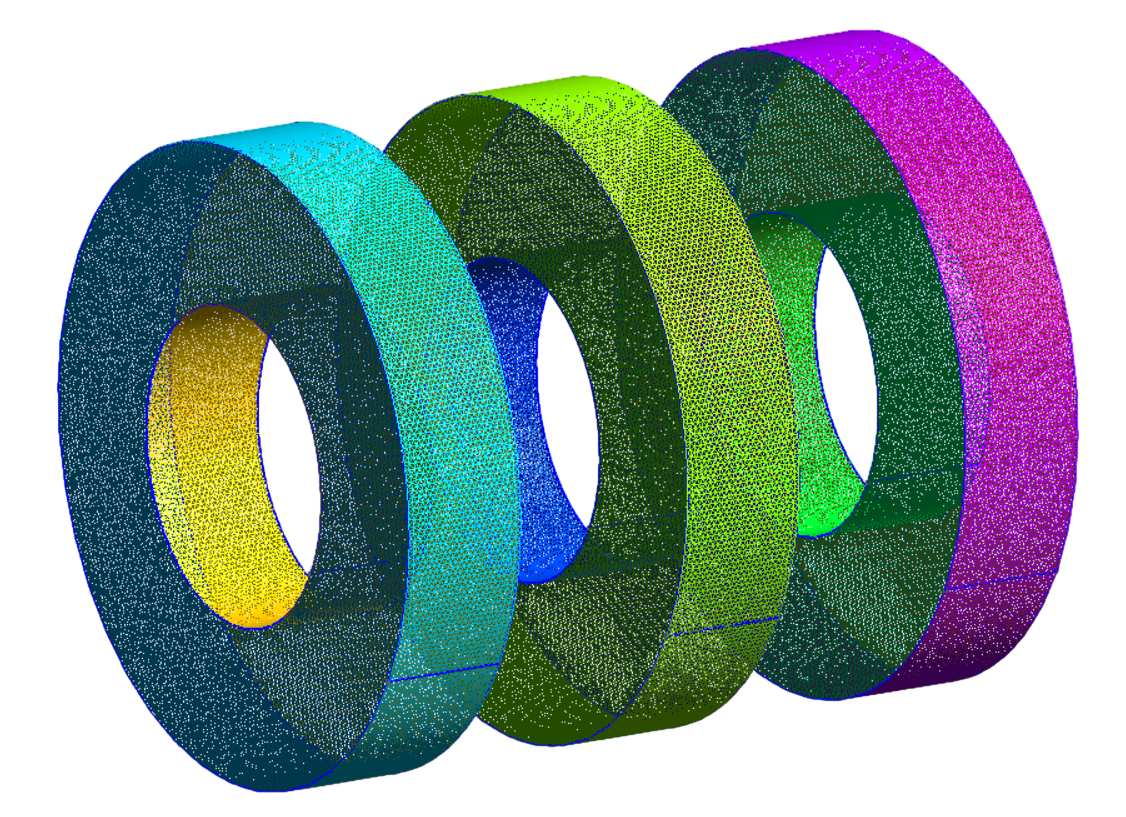
\includegraphics[width=0.4\linewidth]{images/Maillage Einzel.png} 
\caption{Maillage de lentille de Einzel avec Gmsh}
\label{fig:maillage_einzel}
\end{figure}

Une fois cette bibliothèque Pyhton maitrisée, nous avons pu passer à la modélisation et au maillage du quadrupole d'Okayama. Celui-ci est composé
de trois parties différentes: les électrodes cylindriques, les apertures circulaires et le shield. {(\color{red} doit on mettre ces mots en français?)}
Au centre du quadrupole se situent les quatres électrodes cylindriques. Celle-ci sont polarisées inversement polarisée par paires: toutes les électrodes
ont le même potentiel à un signe près. Ces électrodes permettent de focaliser le rayon selon une direction et le défocaliser selon une autre.
Les apertures servent à {(\color{red} je sais pas quoi dire ici)}
Le shield quand à lui sert à isoler le quadrupole afin de représenter un système réaliste car le quadrupole est toujours enfermé dans la colonne de 
l'intrument sur lequel il est installé. 

\begin{figure}[H]
\centering
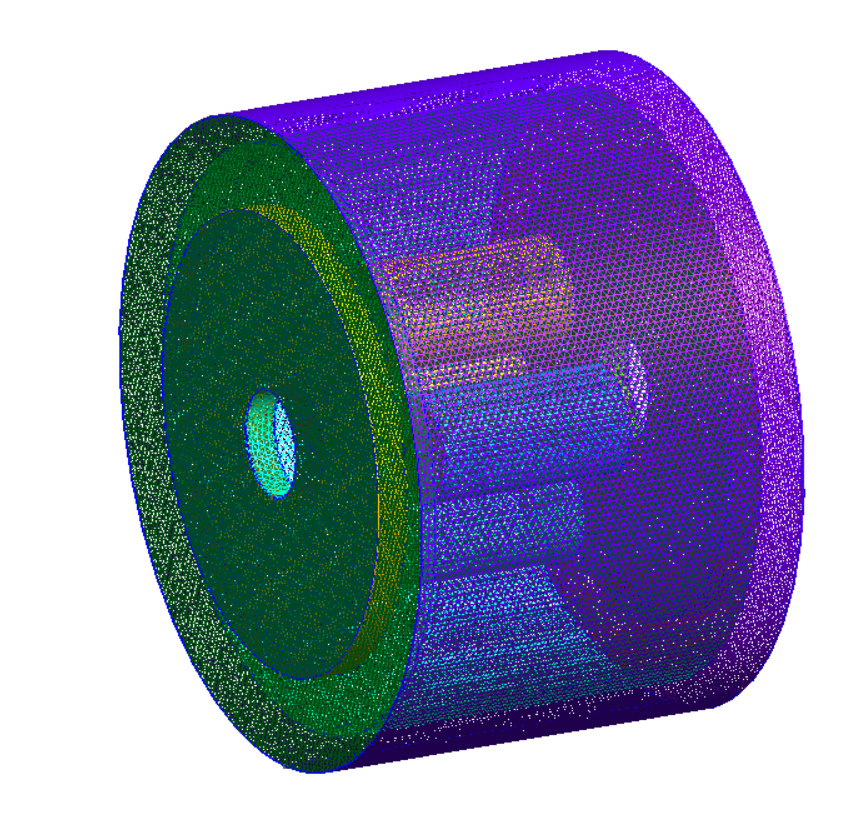
\includegraphics[width=0.3\linewidth]{images/Maillage de biais incliné.png} 
\caption{Maillage du quadrupole (vue complète)}
\label{fig:maillage_quad_complet}
\end{figure}

\begin{figure}[H]
\centering

\begin{minipage}{0.4\textwidth}
    \centering
    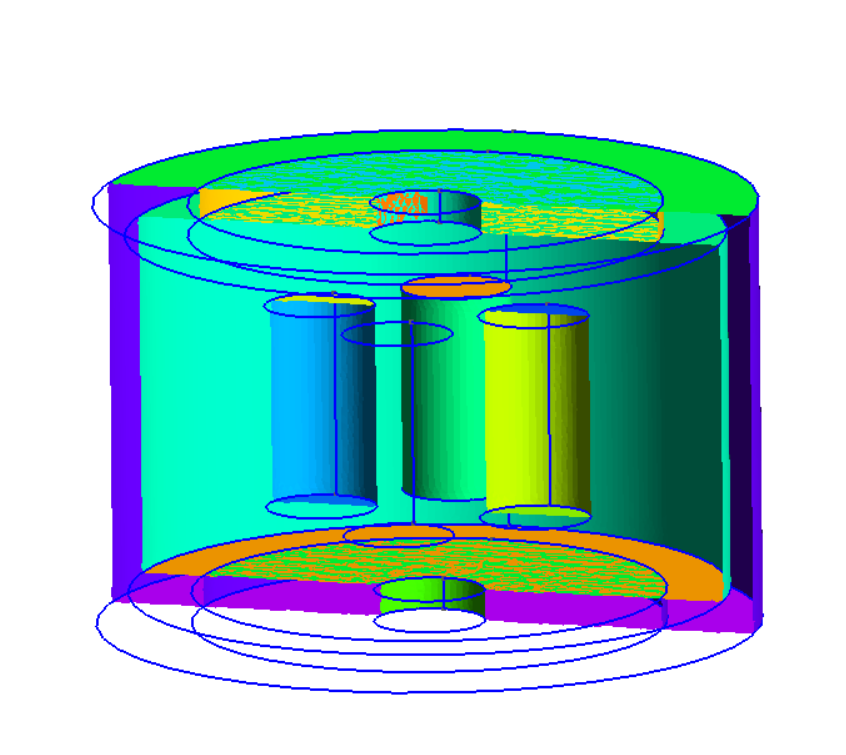
\includegraphics[width=\linewidth]{images/Coupe en longueur.png}
    \caption{Vue en coupe dans la longueur du quadrupole}
    \label{fig:coupe_quad}
\end{minipage}
\hspace{2cm}
\begin{minipage}{0.4\textwidth}
    \centering
    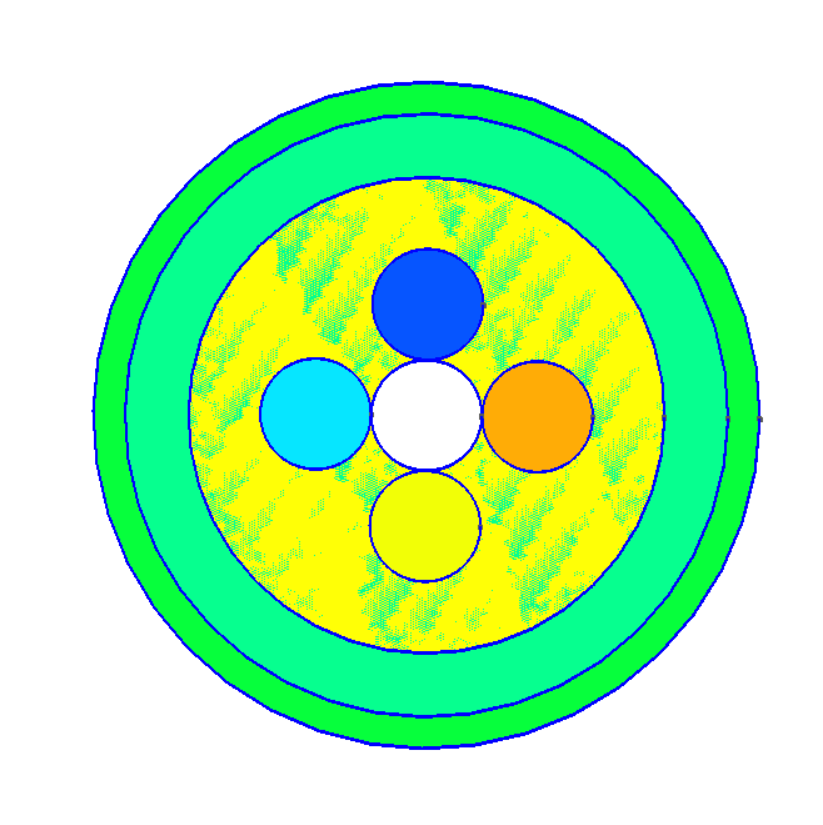
\includegraphics[width=\linewidth]{images/Coupe de face.png}
    \caption{Vue en coupe de face du quadrupole}
    \label{fig:shield_quad}
\end{minipage}

\end{figure}


Une fois la modélisation de la géométrie effectuée, la bibliothèque Python maille les surfaces de cette géométrie. Le maillage est nécessaire car
il permet d'appliquer la méthode des éléments de frontières. 

\section{Méthode des éléments de frontière}
La "Boundary Element Method" ou bien en français la Méthode des éléments de frontière \cite{}

\chapter{Bibliographie}
\printbibliography

\end{document}